\documentclass[]{tufte-handout}

% ams
\usepackage{amssymb,amsmath}

\usepackage{ifxetex,ifluatex}
\usepackage{fixltx2e} % provides \textsubscript
\ifnum 0\ifxetex 1\fi\ifluatex 1\fi=0 % if pdftex
  \usepackage[T1]{fontenc}
  \usepackage[utf8]{inputenc}
\else % if luatex or xelatex
  \makeatletter
  \@ifpackageloaded{fontspec}{}{\usepackage{fontspec}}
  \makeatother
  \defaultfontfeatures{Ligatures=TeX,Scale=MatchLowercase}
  \makeatletter
  \@ifpackageloaded{soul}{
     \renewcommand\allcapsspacing[1]{{\addfontfeature{LetterSpace=15}#1}}
     \renewcommand\smallcapsspacing[1]{{\addfontfeature{LetterSpace=10}#1}}
   }{}
  \makeatother

\fi

% graphix
\usepackage{graphicx}
\setkeys{Gin}{width=\linewidth,totalheight=\textheight,keepaspectratio}

% booktabs
\usepackage{booktabs}

% url
\usepackage{url}

% hyperref
\usepackage{hyperref}

% units.
\usepackage{units}


\setcounter{secnumdepth}{-1}

% citations

% pandoc syntax highlighting

% longtable

% multiplecol
\usepackage{multicol}

% strikeout
\usepackage[normalem]{ulem}

% morefloats
\usepackage{morefloats}


% tightlist macro required by pandoc >= 1.14
\providecommand{\tightlist}{%
  \setlength{\itemsep}{0pt}\setlength{\parskip}{0pt}}

% title / author / date
\date{}


\begin{document}





\thispagestyle{empty}

\LARGE \emph{Perdue Property}\\
\Large \emph{Forest Management Plan}\\
\Large \emph{January 13, 2020}

\begin{marginfigure}

{\centering 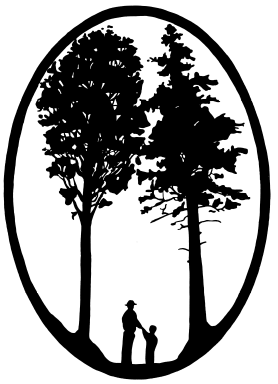
\includegraphics[width=0.3\linewidth,height=0.3\textheight]{C:/Users/Neal/projects/cruise/logo-small} 

}

\end{marginfigure}

\normalsize 

\begin{marginfigure}
\noindent \textit{\large Prepared by} 
\newline\indent Neal F. Maker and John D. Foppert  
\newline\indent Pekin Branch Forestry  
\newline\indent 1324 West County Road  
\newline\indent Calais, VT 05648  
\newline\indent (802) 229-9757  
\end{marginfigure}

\begin{marginfigure}
\noindent \textit{\large Owner}
\newline\indent Holly Perdue and Frances Rousseau  
\newline\indent 101 Harris Hill Road
\indent 
\newline\indent Worcester, VT 05682  
\end{marginfigure}

\begin{marginfigure}
\noindent \textit{\large Property}   
\newline\indent 295 acres and two dwellings   
\newline\indent Worcester, VT  
\newline\indent SPAN 788-251-10339  
\newline\indent Map delineation based on VMP  
\newline\indent Photo(s) 148212, 148208  
\end{marginfigure}

\begin{marginfigure}
\noindent \textit{\large Effective date of plan}  
\newline\indent April 1, 2020  
\end{marginfigure}

\vspace{30pt} \indent This forest management plan is a blueprint for
responsible land stewardship. It is the result of a planning process
that incorporated an assessment of the history and current conditions on
the property, consideration of the various courses of future development
that the forest could follow, and discernment as to which outcomes best
suit my particular objectives (Leak, Yamasaki, and Holleran 2014).

\vspace{5pt} By signing below, I certify that I approve of---and agree
to manage my forestland according to---the following management plan. I
further certify that any of my forestland that is enrolled in Vermont's
Use Value Appraisal program is under active long-term forest management
in accordance with the state's minimum acceptable standards for forest
management. These standards include following Acceptable Management
Practices to maintain water quality on logging operations.

\vspace{38pt}

\noindent\rule{9cm}{0.4pt} \rule{.3cm}{0pt} \rule{4cm}{0.4pt}

\noindent Landowner \rule{7.7cm}{0pt} Date

\vspace{18pt}

\noindent\rule{9cm}{0.4pt} \rule{.3cm}{0pt} \rule{4cm}{0.4pt}

\noindent Landowner \rule{7.7cm}{0pt} Date

\vspace{18pt}

\noindent\rule{9cm}{0.4pt} \rule{.3cm}{0pt} \rule{4cm}{0.4pt}

\noindent Landowner \rule{7.7cm}{0pt} Date

\vspace{18pt}

\noindent\rule{9cm}{0.4pt} \rule{.3cm}{0pt} \rule{4cm}{0.4pt}

\noindent Landowner \rule{7.7cm}{0pt} Date

\vspace{24pt}

This forest management plan meets the standards promulgated by the
Vermont Department of Forests, Parks and Recreation as required for
eligibility in the Use Value Appraisal Program.

\vspace{22pt}

\noindent\rule{9cm}{0.4pt} \rule{.3cm}{0pt} \rule{4cm}{0.4pt}

\noindent County Forester \rule{7cm}{0pt} Date

\pagebreak

\section{Introduction}\label{introduction}

This plan Covers the ten year period from 2020 to 2029. It lays out the
near- and medium-term actions that should guide the development of the
Perdue Forest. It also qualifies the property for Use Value Appraisal
(UVA) and commensurate reduction in property taxes.\footnote{Further
  information about UVA and current valuations can be found at the
  Vermont Tax Department's website:
  \url{https://tax.vermont.gov/property-owners/current-use}.
  \vspace{20pt}} Owners participating in the Use Value Appraisal program
are obliged to manage their property according to the plan and to make
any reasonable investments for improvement that the plan
recommends.\footnote{UVA management plan standards are determined by the
  Department of Forests, Parks, \& Recreation and are available at
  \url{https://fpr.vermont.gov/forest/your_woods/use_value_appraisal} or
  through a County Forester.} Its recommendations were developed in
accordance with the principles and practices of scientifically sound
forestry, as described in the relevant management guidelines, textbooks
and academic journals.

\section{Property Description}\label{property-description}

Some 2 percent of the 295 acre Perdue property is productive forestland
that will be managed according to this plan. Its elevations range from
1110 to 1480 feet above mean sea level. NA NA Soils, forest health, and
other pertinent topics are discussed in the individual stand area
descriptions that follow.

\section{Principles, Goals \& Strategies For Forest
Management}\label{principles-goals-strategies-for-forest-management}

\subsection{Ecological integrity, wildlife habitat, and
biodiversity}\label{ecological-integrity-wildlife-habitat-and-biodiversity}

Management should prioritize the protection of critical ecological
functions, water resources, and threatened or rare plant and wildlife
communities. Wetlands and stream-side riparian zones should be carefully
delineated and protected; and management should give consideration to
the habitat needs of native wildlife populations and to the relationship
between the property, its neighbors and the larger landscape they are
nested within. Management should be informed by and aim to improve
landscape diversity, wildlife travel corridors, and habitat
connectivity. Locally under-represented habitat types should be
identified and promoted. Stand scale and sub-stand scale management
should focus on developing or maintaining species-specific habitat
needs, such as nesting sites, cover, mast production, preferred browse
or other unique structural and compositional requirements.

\subsection{Timber management}\label{timber-management}

Management should provide regular returns from timber harvesting.
Long-term value growth is provided by maintaining full site occupancy
with investment-grade stems: healthy trees capable of producing high
quality sawtimber or veneer and worth retaining in the stand until they
reach their full, site- and species-specific target diameters. Tree
species which yield sought-after, high-value wood should be promoted
within each stand or, when regenerating a new stand, attention should be
paid to providing the stand conditions which favor the establishment of
those species. At a property-wide scale, a variety of species should be
maintained, providing options for seizing future market opportunities
and a hedge against species-specific market depreciation. Among desired
species, additional preference should be given to individual trees of
sufficient vigor and grade-potential for strong future value growth.
Consideration of economic efficiency should inform the timing and
coordination of infrastructure investments and stand maintenance,
improvement and harvest operations.

\section{Stand Descriptions \& Management
Recommendations}\label{stand-descriptions-management-recommendations}

\begin{marginfigure} \noindent \textit{\LARGE Management Schedule} 

 \vspace{10 pt} 

 \noindent \textit{\large 2023} 

 \begin{itemize} \item Area 1: Group Selection 

 \item Area 3: Continuous Cover Irregular Shelterwood 

 \item Area 4: Precommercial Thinning 

 \item Area 5: Continuous Cover Irregular Shelterwood 

 \item Area 6: Group Selection 

 \item Area 7: Hybrid Selection 

 \end{itemize} \vspace{10 pt} 

 \noindent \textit{\large 2029} 

 \begin{itemize} \item Reinventory forest 

 \end{itemize} \end{marginfigure}

Presented below are detailed stand-by-stand descriptions of the forest,
the long-term structural, compositional and functional goals for each
stand, and the near-term silvicultural treatments or management
activities that have been prescribed to advance each stand toward those
goals. The data presented in the following pages was obtained from a
field examination of the property in September of 2019. General
conditions were assessed qualitatively in conjunction with quantitative
sampling. Observational notes and sample summary statistics together
provide the basis for the area descriptions and management
recommendations. All sampling was done using a systematic sample and
variable radius plots. In stands with uneven-aged structures, all trees
6" dbh and larger were measured in each plot. In stands with even-aged
structures, all main-canopy trees were measured in each plot.

When contractors are used to implement silvicultural prescriptions, they
should be highly skilled, properly equipped, fully insured, and closely
supervised. A professional forester should prepare and administer
commercial treatments, and logging operations should be timed to
coincide with favorable weather conditions (working on wet soils only
when they are frozen, for instance) and favorable timber markets. Use
Value Appraisal program guidelines allow any management activities
prescribed in this plan to be carried out up to three years before or
after the date indicated. Landowners in the Use Value Appraisal program
must file a Forest Management Activity Report with the County Forester
by February 1\textsuperscript{st} if any commercial logging occurred in
the previous year.

The property should be reinventoried in 2029 and the findings brought to
bear on a reassessment of the goals and strategies proposed in this
plan, leading to a formal management plan update. At any point over the
course of this management period, this plan may be updated to
incorporate new information and to reflect any new thoughts, concerns or
considerations on the part of the family or the foresters helping to
manage their land.

\newpage

\section{Area 1}\label{area-1}

Northern hardwood\\
\noindent 1.00 legal acres \textbar{} 1.00 measured acres

\subsection{Site-specific information}\label{site-specific-information}

\begin{quote}
\begin{itemize}
\tightlist
\item
  \textbf{Soils:}\\
  \indent\indent  NA
\end{itemize}
\end{quote}

\begin{quote}
\begin{itemize}
\tightlist
\item
  \textbf{Site Class:}\\
  \vspace{2pt} II (determined from soil mapping and field assessment)
\end{itemize}
\end{quote}

\begin{quote}
\begin{itemize}
\tightlist
\item
  \textbf{Access:}\\
  \vspace{2pt} Good. Less than 1 mile
\end{itemize}
\end{quote}

\begin{quote}
\begin{itemize}
\tightlist
\item
  \textbf{Stand history:}\\
  \vspace{2pt} Established c. 1940, possibly from abandoned pasture.
  Highgraded, most recently c. 1990.
\end{itemize}
\end{quote}

\subsection{Current forest
information}\label{current-forest-information}

\begin{quote}
\begin{itemize}
\tightlist
\item
  \textbf{Age Class Structure:}\\
  \vspace{2pt} Even-aged\\

  \begin{marginfigure}
  \includegraphics{fmp-vt_files/figure-latex/unnamed-chunk-2-1} \caption[Distributions are approximated with kernel density estimation]{Distributions are approximated with kernel density estimation. Common species are those that account for at least 8 percent of the total stocking and areas under each curve represent species basal areas.}\label{fig:unnamed-chunk-2}
  \end{marginfigure}
\end{itemize}
\end{quote}

\begin{quote}
\begin{itemize}
\tightlist
\item
  \textbf{Species (\% stocking):}\\
  \vspace{2pt} hard maple (28\%), soft maple (20\%), yellow birch
  (15\%), ash (14\%), beech (12\%), hemlock (7\%), red oak (2\%), black
  cherry (1\%), paper birch (1\%), spruce (1\%)
\end{itemize}
\end{quote}

\begin{quote}
\begin{itemize}
\tightlist
\item
  \textbf{Regeneration:}\\
  \vspace{2pt} Well established beech understory.
\end{itemize}
\end{quote}

\begin{quote}
\begin{itemize}
\tightlist
\item
  \textbf{Forest health:}\\
  \vspace{2pt} Beech bark disease (probably coupled with high deer
  browse pressure) is a severe impediment to regeneration. Overstory
  health and quality are low because of past highgrading. No exotic
  invasives noted.
\end{itemize}
\end{quote}

\begin{quote}
\begin{itemize}
\tightlist
\item
  \textbf{Standing dead wood (sq ft/ac by size class):}\\
  \vspace{2pt} \indent \small 6-10``: 5.5 \textbar{} 11-16'': 1.8
  \textbar{} 17-22'': 0.9 \textbar{} 23+'': 0
\end{itemize}
\end{quote}

\subsection{Inventory information}\label{inventory-information}

\begin{quote}
\begin{itemize}
\tightlist
\item
  11 points, 10 BAF, September, 2019
\end{itemize}
\end{quote}

\begin{figure}
\includegraphics{fmp-vt_files/figure-latex/unnamed-chunk-5-1} \caption[Points represent individual plots]{Points represent individual plots. Asterisk represnts stand average. Radial lines are quadratic stand diameters.}\label{fig:unnamed-chunk-5}
\end{figure}

\begin{table}

\caption{\label{tab:unnamed-chunk-6}Measures of stocking for all live trees (Total), acceptable growing stock (AGS), and unacceptable growing stock (UGS).}
\centering
\begin{tabular}[t]{lrrr}
\toprule
Measure & Total & AGS & UGS\\
\midrule
Basal area (sq ft/ac) & 119 & 77 & 42\\
QSD (in) & 11 & 11 & 11\\
Stems/ac & 174 & 108 & 66\\
\bottomrule
\end{tabular}
\end{table}

\begin{table}

\caption{\label{tab:unnamed-chunk-7}Current basal area (sq ft/ac) of total growing stock, acceptable growing stock, and unacceptable growing stock by size class.}
\centering
\begin{tabular}[t]{lrrr}
\toprule
Size Class & Total & AGS & UGS\\
\midrule
6-11 in. & 49 & 30 & 19\\
12-15 in. & 52 & 39 & 13\\
16-21 in. & 15 & 7 & 8\\
22+ in. & 3 & 1 & 2\\
Total & 119 & 77 & 42\\
\bottomrule
\end{tabular}
\end{table}

\subsection{Long-term management
system}\label{long-term-management-system}

\textbf{NA}

NA

\subsection{Silvicultural
prescription}\label{silvicultural-prescription}

\textbf{Group Selection}\\
\noindent \textbf{Year:} 2023

clear-cut \& treat beech, groups and treat beech, avoid dealing with.

\newpage

\section{Area 2}\label{area-2}

White pine\\
\noindent 1.00 legal acres \textbar{} 1.00 measured acres

\subsection{Site-specific
information}\label{site-specific-information-1}

\begin{quote}
\begin{itemize}
\tightlist
\item
  \textbf{Soils:}\\
  \indent\indent  NA
\end{itemize}
\end{quote}

\begin{quote}
\begin{itemize}
\tightlist
\item
  \textbf{Site Class:}\\
  \vspace{2pt} II (determined from soil mapping and field assessment)
\end{itemize}
\end{quote}

\begin{quote}
\begin{itemize}
\tightlist
\item
  \textbf{Access:}\\
  \vspace{2pt} Excellent. Less than one mile.
\end{itemize}
\end{quote}

\begin{quote}
\begin{itemize}
\tightlist
\item
  \textbf{Stand history:}\\
  \vspace{2pt} Previous plan reports the area as pasture land that was
  abandoned c. 1950. We suspect abandonment was more like 1930. Well
  tended through several thinnings, around 1995 and in 2001.
\end{itemize}
\end{quote}

\subsection{Current forest
information}\label{current-forest-information-1}

\begin{quote}
\begin{itemize}
\tightlist
\item
  \textbf{Age Class Structure:}\\
  \vspace{2pt} Two-aged\\

  \begin{marginfigure}
  \includegraphics{fmp-vt_files/figure-latex/unnamed-chunk-8-1} \caption[Distributions are approximated with kernel density estimation]{Distributions are approximated with kernel density estimation. Common species are those that account for at least 8 percent of the total stocking and areas under each curve represent species basal areas.}\label{fig:unnamed-chunk-8}
  \end{marginfigure}
\end{itemize}
\end{quote}

\begin{quote}
\begin{itemize}
\tightlist
\item
  \textbf{Species (\% stocking):}\\
  \vspace{2pt} white pine (51\%), soft maple (31\%), spruce (18\%)
\end{itemize}
\end{quote}

\begin{quote}
\begin{itemize}
\tightlist
\item
  \textbf{Regeneration:}\\
  \vspace{2pt} Abundant fir, soft maple, striped maple, and black cherry
  in most areas. Other valuable hardwoods (including red oak) are
  present as seedlings.
\end{itemize}
\end{quote}

\begin{quote}
\begin{itemize}
\tightlist
\item
  \textbf{Forest health:}\\
  \vspace{2pt} Very few diseases in pines. Soft maple is of mixed
  quality. No exotic invasives noted.
\end{itemize}
\end{quote}

\begin{quote}
\begin{itemize}
\tightlist
\item
  \textbf{Standing dead wood (sq ft/ac by size class):}\\
  \vspace{2pt} \indent \small 6-10``: 5 \textbar{} 11-16'': 0 \textbar{}
  17-22'': 0 \textbar{} 23+'': 0
\end{itemize}
\end{quote}

\subsection{Inventory information}\label{inventory-information-1}

\begin{quote}
\begin{itemize}
\tightlist
\item
  4 points, 10 BAF, September, 2019
\end{itemize}
\end{quote}

\begin{figure}
\includegraphics{fmp-vt_files/figure-latex/unnamed-chunk-11-1} \caption[Points represent individual plots]{Points represent individual plots. Asterisk represnts stand average. Radial lines are quadratic stand diameters.}\label{fig:unnamed-chunk-11}
\end{figure}

\begin{table}

\caption{\label{tab:unnamed-chunk-12}Measures of stocking for all live trees (Total), acceptable growing stock (AGS), and unacceptable growing stock (UGS).}
\centering
\begin{tabular}[t]{lrrr}
\toprule
Measure & Total & AGS & UGS\\
\midrule
Basal area (sq ft/ac) & 112 & 90 & 22\\
QSD (in) & 12 & 13 & 11\\
Stems/ac & 135 & 98 & 37\\
\bottomrule
\end{tabular}
\end{table}

\begin{table}

\caption{\label{tab:unnamed-chunk-13}Current basal area (sq ft/ac) of total growing stock, acceptable growing stock, and unacceptable growing stock by size class.}
\centering
\begin{tabular}[t]{lrrr}
\toprule
Size Class & Total & AGS & UGS\\
\midrule
6-11 in. & 32 & 25 & 8\\
12-15 in. & 28 & 15 & 12\\
16-21 in. & 35 & 32 & 2\\
22+ in. & 18 & 18 & 0\\
Total & 112 & 90 & 22\\
\bottomrule
\end{tabular}
\end{table}

\subsection{Long-term management
system}\label{long-term-management-system-1}

\textbf{NA}

NA

\subsection{Silvicultural
prescription}\label{silvicultural-prescription-1}

NA

\newpage

\section{Area 3}\label{area-3}

Mixedwood\\
\noindent 1.00 legal acres \textbar{} 1.00 measured acres

\subsection{Site-specific
information}\label{site-specific-information-2}

\begin{quote}
\begin{itemize}
\tightlist
\item
  \textbf{Soils:}\\
  \indent\indent  NA
\end{itemize}
\end{quote}

\begin{quote}
\begin{itemize}
\tightlist
\item
  \textbf{Site Class:}\\
  \vspace{2pt} II (determined from soil mapping and field assessment)
\end{itemize}
\end{quote}

\begin{quote}
\begin{itemize}
\tightlist
\item
  \textbf{Access:}\\
  \vspace{2pt} Fair. Less than one mile.
\end{itemize}
\end{quote}

\begin{quote}
\begin{itemize}
\tightlist
\item
  \textbf{Stand history:}\\
  \vspace{2pt} Probably continuously forested. Periodic logging.
  Highgraded c. 1990.
\end{itemize}
\end{quote}

\subsection{Current forest
information}\label{current-forest-information-2}

\begin{quote}
\begin{itemize}
\tightlist
\item
  \textbf{Age Class Structure:}\\
  \vspace{2pt} Uneven-aged\\

  \begin{marginfigure}
  \includegraphics{fmp-vt_files/figure-latex/unnamed-chunk-14-1} \caption[Distributions are approximated with kernel density estimation]{Distributions are approximated with kernel density estimation. Common species are those that account for at least 8 percent of the total stocking and areas under each curve represent species basal areas.}\label{fig:unnamed-chunk-14}
  \end{marginfigure}
\end{itemize}
\end{quote}

\begin{quote}
\begin{itemize}
\tightlist
\item
  \textbf{Species (\% stocking):}\\
  \vspace{2pt} soft maple (46\%), hemlock (33\%), fir (10\%), spruce
  (5\%), hard maple (3\%), white pine (3\%)
\end{itemize}
\end{quote}

\begin{quote}
\begin{itemize}
\tightlist
\item
  \textbf{Regeneration:}\\
  \vspace{2pt} Well established fir and spruce, except where stocking
  rains high.
\end{itemize}
\end{quote}

\begin{quote}
\begin{itemize}
\tightlist
\item
  \textbf{Forest health:}\\
  \vspace{2pt} Generally poor quality because of highgrading. No exotic
  invasives noted.
\end{itemize}
\end{quote}

\begin{quote}
\begin{itemize}
\tightlist
\item
  \textbf{Standing dead wood (sq ft/ac by size class):}\\
  \vspace{2pt} \indent \small 6-10``: 3.3 \textbar{} 11-16'': 3.3
  \textbar{} 17-22'': 0 \textbar{} 23+'': 3.3
\end{itemize}
\end{quote}

\subsection{Inventory information}\label{inventory-information-2}

\begin{quote}
\begin{itemize}
\tightlist
\item
  3 points, 10 BAF, September, 2019
\end{itemize}
\end{quote}

\begin{figure}
\includegraphics{fmp-vt_files/figure-latex/unnamed-chunk-17-1} \caption[Points represent individual plots]{Points represent individual plots. Asterisk represnts stand average. Radial lines are quadratic stand diameters.}\label{fig:unnamed-chunk-17}
\end{figure}

\begin{table}

\caption{\label{tab:unnamed-chunk-18}Measures of stocking for all live trees (Total), acceptable growing stock (AGS), and unacceptable growing stock (UGS).}
\centering
\begin{tabular}[t]{lrrr}
\toprule
Measure & Total & AGS & UGS\\
\midrule
Basal area (sq ft/ac) & 130 & 110 & 20\\
QSD (in) & 12 & 12 & 13\\
Stems/ac & 173 & 152 & 21\\
\bottomrule
\end{tabular}
\end{table}

\begin{table}

\caption{\label{tab:unnamed-chunk-19}Current (total, acceptable, and unacceptable growing stock) and post-harvest target basal areas (sq ft/ac) by size class.}
\centering
\begin{tabular}[t]{lrrrr}
\toprule
Size Class & Total & AGS & UGS & Target\\
\midrule
6-11 in. & 50 & 43 & 7 & 30\\
12-15 in. & 60 & 53 & 7 & 30\\
16-21 in. & 13 & 13 & 0 & 25\\
22+ in. & 7 & 0 & 7 & 15\\
Total & 130 & 110 & 20 & 100\\
\bottomrule
\end{tabular}
\end{table}

\subsection{Long-term management
system}\label{long-term-management-system-2}

\textbf{NA}

NA

\subsection{Silvicultural
prescription}\label{silvicultural-prescription-2}

\textbf{Continuous Cover Irregular Shelterwood}\\
\noindent \textbf{Year:} 2023

Group and individual tree selection with focus on quality.

\newpage

\section{Area 4}\label{area-4}

Mixedwood\\
\noindent 1.00 legal acres \textbar{} 1.00 measured acres

\subsection{Site-specific
information}\label{site-specific-information-3}

\begin{quote}
\begin{itemize}
\tightlist
\item
  \textbf{Soils:}\\
  \indent\indent  NA
\end{itemize}
\end{quote}

\begin{quote}
\begin{itemize}
\tightlist
\item
  \textbf{Site Class:}\\
  \vspace{2pt} II (determined from soil mapping and field assessment)
\end{itemize}
\end{quote}

\begin{quote}
\begin{itemize}
\tightlist
\item
  \textbf{Access:}\\
  \vspace{2pt} Good access from adjacent fields. Less than one mile.
\end{itemize}
\end{quote}

\begin{quote}
\begin{itemize}
\tightlist
\item
  \textbf{Stand history:}\\
  \vspace{2pt} Progressive pasture abandonment. Western edge abandoned
  c. 1930s. Occasional grazing elsewhere until early 1980s.
\end{itemize}
\end{quote}

\subsection{Current forest
information}\label{current-forest-information-3}

\begin{quote}
\begin{itemize}
\tightlist
\item
  \textbf{Age Class Structure:}\\
  \vspace{2pt} Even-aged\\

  \begin{marginfigure}
  \includegraphics{fmp-vt_files/figure-latex/unnamed-chunk-20-1} \caption[Distributions are approximated with kernel density estimation]{Distributions are approximated with kernel density estimation. Common species are those that account for at least 8 percent of the total stocking and areas under each curve represent species basal areas.}\label{fig:unnamed-chunk-20}
  \end{marginfigure}
\end{itemize}
\end{quote}

\begin{quote}
\begin{itemize}
\tightlist
\item
  \textbf{Species (\% stocking):}\\
  \vspace{2pt} soft maple (24\%), fir (23\%), white pine (23\%), spruce
  (10\%), hard maple (5\%), ash (4\%), aspen (3\%), yellow birch (3\%),
  other hardwood (2\%), beech (1\%), paper birch (1\%)
\end{itemize}
\end{quote}

\begin{quote}
\begin{itemize}
\tightlist
\item
  \textbf{Regeneration:}\\
  \vspace{2pt} Most of stand is still in stem exclusion stage.
\end{itemize}
\end{quote}

\begin{quote}
\begin{itemize}
\tightlist
\item
  \textbf{Forest health:}\\
  \vspace{2pt} Many pines are poorly formed, especially where grazing
  continued. Blister rust present on some pines. No exotic invasives
  noted.
\end{itemize}
\end{quote}

\begin{quote}
\begin{itemize}
\tightlist
\item
  \textbf{Standing dead wood (sq ft/ac by size class):}\\
  \vspace{2pt} \indent \small 6-10``: 4.3 \textbar{} 11-16'': 7.1
  \textbar{} 17-22'': 0 \textbar{} 23+'': 1.4
\end{itemize}
\end{quote}

\subsection{Inventory information}\label{inventory-information-3}

\begin{quote}
\begin{itemize}
\tightlist
\item
  7 points, 10 BAF, September, 2019
\end{itemize}
\end{quote}

\begin{figure}
\includegraphics{fmp-vt_files/figure-latex/unnamed-chunk-23-1} \caption[Points represent individual plots]{Points represent individual plots. Asterisk represnts stand average. Radial lines are quadratic stand diameters.}\label{fig:unnamed-chunk-23}
\end{figure}

\begin{table}

\caption{\label{tab:unnamed-chunk-24}Measures of stocking for all live trees (Total), acceptable growing stock (AGS), and unacceptable growing stock (UGS).}
\centering
\begin{tabular}[t]{lrrr}
\toprule
Measure & Total & AGS & UGS\\
\midrule
Basal area (sq ft/ac) & 137 & 109 & 28\\
QSD (in) & 10 & 10 & 11\\
Stems/ac & 232 & 188 & 44\\
\bottomrule
\end{tabular}
\end{table}

\begin{table}

\caption{\label{tab:unnamed-chunk-25}Current basal area (sq ft/ac) of total growing stock, acceptable growing stock, and unacceptable growing stock by size class.}
\centering
\begin{tabular}[t]{lrrr}
\toprule
Size Class & Total & AGS & UGS\\
\midrule
6-11 in. & 57 & 49 & 9\\
12-15 in. & 43 & 34 & 9\\
16-21 in. & 27 & 17 & 10\\
22+ in. & 10 & 9 & 1\\
Total & 137 & 109 & 29\\
\bottomrule
\end{tabular}
\end{table}

\subsection{Long-term management
system}\label{long-term-management-system-3}

\textbf{NA}

NA

\subsection{Silvicultural
prescription}\label{silvicultural-prescription-3}

\textbf{Precommercial Thinning}\\
\noindent \textbf{Year:} 2023

Precommercial release or wait.

\newpage

\section{Area 5}\label{area-5}

Pine-hardwood\\
\noindent 1.00 legal acres \textbar{} 1.00 measured acres

\subsection{Site-specific
information}\label{site-specific-information-4}

\begin{quote}
\begin{itemize}
\tightlist
\item
  \textbf{Soils:}\\
  \indent\indent  NA
\end{itemize}
\end{quote}

\begin{quote}
\begin{itemize}
\tightlist
\item
  \textbf{Site Class:}\\
  \vspace{2pt} III (determined from soil mapping and field assessment)
\end{itemize}
\end{quote}

\begin{quote}
\begin{itemize}
\tightlist
\item
  \textbf{Access:}\\
  \vspace{2pt} Steep ledgy terrain limits maneuverability, but skid
  roads are established in many areas. Small landing located on Eagle
  Ledge Road.
\end{itemize}
\end{quote}

\begin{quote}
\begin{itemize}
\tightlist
\item
  \textbf{Stand history:}\\
  \vspace{2pt} Continuously forested with occasional logging, most
  recently in . Older cohort appears to date to c. 1920.
\end{itemize}
\end{quote}

\subsection{Current forest
information}\label{current-forest-information-4}

\begin{quote}
\begin{itemize}
\tightlist
\item
  \textbf{Age Class Structure:}\\
  \vspace{2pt} Two-aged\\

  \begin{marginfigure}
  \includegraphics{fmp-vt_files/figure-latex/unnamed-chunk-26-1} \caption[Distributions are approximated with kernel density estimation]{Distributions are approximated with kernel density estimation. Common species are those that account for at least 8 percent of the total stocking and areas under each curve represent species basal areas.}\label{fig:unnamed-chunk-26}
  \end{marginfigure}
\end{itemize}
\end{quote}

\begin{quote}
\begin{itemize}
\tightlist
\item
  \textbf{Species (\% stocking):}\\
  \vspace{2pt} soft maple (28\%), hemlock (19\%), spruce (13\%), hard
  maple (12\%), fir (9\%), yellow birch (7\%), ash (4\%), paper birch
  (4\%), aspen (1\%), hophornbeam (1\%), red pine (1\%)
\end{itemize}
\end{quote}

\begin{quote}
\begin{itemize}
\tightlist
\item
  \textbf{Regeneration:}\\
  \vspace{2pt} Spruce, fir, and/or beech fairly well established in most
  places.
\end{itemize}
\end{quote}

\begin{quote}
\begin{itemize}
\tightlist
\item
  \textbf{Forest health:}\\
  \vspace{2pt} Beech are impeding regeneration in places. No exotic
  invasives noted.
\end{itemize}
\end{quote}

\begin{quote}
\begin{itemize}
\tightlist
\item
  \textbf{Standing dead wood (sq ft/ac by size class):}\\
  \vspace{2pt} \indent \small 6-10``: 10 \textbar{} 11-16'': 12.2
  \textbar{} 17-22'': 0 \textbar{} 23+'': 0
\end{itemize}
\end{quote}

\subsection{Inventory information}\label{inventory-information-4}

\begin{quote}
\begin{itemize}
\tightlist
\item
  9 points, 10 BAF, September, 2019
\end{itemize}
\end{quote}

\begin{figure}
\includegraphics{fmp-vt_files/figure-latex/unnamed-chunk-29-1} \caption[Points represent individual plots]{Points represent individual plots. Asterisk represnts stand average. Radial lines are quadratic stand diameters.}\label{fig:unnamed-chunk-29}
\end{figure}

\begin{table}

\caption{\label{tab:unnamed-chunk-30}Measures of stocking for all live trees (Total), acceptable growing stock (AGS), and unacceptable growing stock (UGS).}
\centering
\begin{tabular}[t]{lrrr}
\toprule
Measure & Total & AGS & UGS\\
\midrule
Basal area (sq ft/ac) & 109 & 87 & 22\\
QSD (in) & 11 & 11 & 12\\
Stems/ac & 167 & 138 & 29\\
\bottomrule
\end{tabular}
\end{table}

\begin{table}

\caption{\label{tab:unnamed-chunk-31}Current (total, acceptable, and unacceptable growing stock) and post-harvest target basal areas (sq ft/ac) by size class.}
\centering
\begin{tabular}[t]{lrrrr}
\toprule
Size Class & Total & AGS & UGS & Target\\
\midrule
6-11 in. & 44 & 37 & 8 & 30\\
12-15 in. & 43 & 34 & 9 & 30\\
16-21 in. & 19 & 14 & 4 & 25\\
22+ in. & 2 & 1 & 1 & 15\\
Total & 109 & 87 & 22 & 100\\
\bottomrule
\end{tabular}
\end{table}

\subsection{Long-term management
system}\label{long-term-management-system-4}

\textbf{NA}

NA

\subsection{Silvicultural
prescription}\label{silvicultural-prescription-4}

\textbf{Continuous Cover Irregular Shelterwood}\\
\noindent \textbf{Year:} 2023

Hybrid selection or wait.

\newpage

\section{Area 6}\label{area-6}

Northern hardwood\\
\noindent 1.00 legal acres \textbar{} 1.00 measured acres

\subsection{Site-specific
information}\label{site-specific-information-5}

\begin{quote}
\begin{itemize}
\tightlist
\item
  \textbf{Soils:}\\
  \indent\indent  NA
\end{itemize}
\end{quote}

\begin{quote}
\begin{itemize}
\tightlist
\item
  \textbf{Site Class:}\\
  \vspace{2pt} II (determined from soil mapping and field assessment)
\end{itemize}
\end{quote}

\begin{quote}
\begin{itemize}
\tightlist
\item
  \textbf{Access:}\\
  \vspace{2pt} Probably best accessed from small landing on Eagle Ledge
  road, via steep skid trail. Access from south may be possible too.
\end{itemize}
\end{quote}

\begin{quote}
\begin{itemize}
\tightlist
\item
  \textbf{Stand history:}\\
  \vspace{2pt} Probably pastured some, but never plowed. Oldest trees
  date to c. 1920s. Probably logged several times, most recently in
  2005/06, when mature, declining, and low quality trees were removed.
\end{itemize}
\end{quote}

\subsection{Current forest
information}\label{current-forest-information-5}

\begin{quote}
\begin{itemize}
\tightlist
\item
  \textbf{Age Class Structure:}\\
  \vspace{2pt} Even-aged\\

  \begin{marginfigure}
  \includegraphics{fmp-vt_files/figure-latex/unnamed-chunk-32-1} \caption[Distributions are approximated with kernel density estimation]{Distributions are approximated with kernel density estimation. Common species are those that account for at least 8 percent of the total stocking and areas under each curve represent species basal areas.}\label{fig:unnamed-chunk-32}
  \end{marginfigure}
\end{itemize}
\end{quote}

\begin{quote}
\begin{itemize}
\tightlist
\item
  \textbf{Species (\% stocking):}\\
  \vspace{2pt} soft maple (30\%), yellow birch (19\%), beech (17\%),
  hard maple (11\%), ash (7\%), hemlock (7\%), black cherry (4\%), aspen
  (2\%), paper birch (1\%), spruce (1\%)
\end{itemize}
\end{quote}

\begin{quote}
\begin{itemize}
\tightlist
\item
  \textbf{Regeneration:}\\
  \vspace{2pt} Beech saplings are problematic over most of the stand.
  Limited spruce and fir also present.
\end{itemize}
\end{quote}

\begin{quote}
\begin{itemize}
\tightlist
\item
  \textbf{Forest health:}\\
  \vspace{2pt} Beech bark disease is impeding regeneration. Many
  overstory trees are of marginal quality. No exotic invasives noted.
\end{itemize}
\end{quote}

\begin{quote}
\begin{itemize}
\tightlist
\item
  \textbf{Standing dead wood (sq ft/ac by size class):}\\
  \vspace{2pt} \indent \small 6-10``: 2.9 \textbar{} 11-16'': 10
  \textbar{} 17-22'': 0 \textbar{} 23+'': 0
\end{itemize}
\end{quote}

\subsection{Inventory information}\label{inventory-information-5}

\begin{quote}
\begin{itemize}
\tightlist
\item
  7 points, 10 BAF, September, 2019
\end{itemize}
\end{quote}

\begin{figure}
\includegraphics{fmp-vt_files/figure-latex/unnamed-chunk-35-1} \caption[Points represent individual plots]{Points represent individual plots. Asterisk represnts stand average. Radial lines are quadratic stand diameters.}\label{fig:unnamed-chunk-35}
\end{figure}

\begin{table}

\caption{\label{tab:unnamed-chunk-36}Measures of stocking for all live trees (Total), acceptable growing stock (AGS), and unacceptable growing stock (UGS).}
\centering
\begin{tabular}[t]{lrrr}
\toprule
Measure & Total & AGS & UGS\\
\midrule
Basal area (sq ft/ac) & 119 & 86 & 33\\
QSD (in) & 11 & 12 & 9\\
Stems/ac & 189 & 120 & 69\\
\bottomrule
\end{tabular}
\end{table}

\begin{table}

\caption{\label{tab:unnamed-chunk-37}Current basal area (sq ft/ac) of total growing stock, acceptable growing stock, and unacceptable growing stock by size class.}
\centering
\begin{tabular}[t]{lrrr}
\toprule
Size Class & Total & AGS & UGS\\
\midrule
6-11 in. & 43 & 24 & 19\\
12-15 in. & 44 & 39 & 6\\
16-21 in. & 30 & 23 & 7\\
22+ in. & 1 & 0 & 1\\
Total & 119 & 86 & 33\\
\bottomrule
\end{tabular}
\end{table}

\subsection{Long-term management
system}\label{long-term-management-system-5}

\textbf{NA}

NA

\subsection{Silvicultural
prescription}\label{silvicultural-prescription-5}

\textbf{Group Selection}\\
\noindent \textbf{Year:} 2023

Group selection with beech control or wait.

\newpage

\section{Area 7}\label{area-7}

Mixedwood\\
\noindent 1.00 legal acres \textbar{} 1.00 measured acres

\subsection{Site-specific
information}\label{site-specific-information-6}

\begin{quote}
\begin{itemize}
\tightlist
\item
  \textbf{Soils:}\\
  \indent\indent  NA
\end{itemize}
\end{quote}

\begin{quote}
\begin{itemize}
\tightlist
\item
  \textbf{Site Class:}\\
  \vspace{2pt} II (determined from soil mapping and field assessment)
\end{itemize}
\end{quote}

\begin{quote}
\begin{itemize}
\tightlist
\item
  \textbf{Access:}\\
  \vspace{2pt} One main skid trail provides the only access from a small
  landing on Eagle Ledge road. Wet soils restrict movement at certain
  times of year. Best to enter in dry conditions.
\end{itemize}
\end{quote}

\begin{quote}
\begin{itemize}
\tightlist
\item
  \textbf{Stand history:}\\
  \vspace{2pt} Parts were probably pastured to a limited degree, but
  never plowed. The oldes trees are probably over 100, while the
  majority of the overstory dates to between 1930 and 1950. Logged
  several times, most recently in 2005/06, when soft maple, spruce, and
  fir were targeted.
\end{itemize}
\end{quote}

\subsection{Current forest
information}\label{current-forest-information-6}

\begin{quote}
\begin{itemize}
\tightlist
\item
  \textbf{Age Class Structure:}\\
  \vspace{2pt} Two-aged\\

  \begin{marginfigure}
  \includegraphics{fmp-vt_files/figure-latex/unnamed-chunk-38-1} \caption[Distributions are approximated with kernel density estimation]{Distributions are approximated with kernel density estimation. Common species are those that account for at least 8 percent of the total stocking and areas under each curve represent species basal areas.}\label{fig:unnamed-chunk-38}
  \end{marginfigure}
\end{itemize}
\end{quote}

\begin{quote}
\begin{itemize}
\tightlist
\item
  \textbf{Species (\% stocking):}\\
  \vspace{2pt} soft maple (35\%), hemlock (27\%), hard maple (8\%),
  beech (7\%), fir (7\%), yellow birch (7\%), spruce (5\%), paper birch
  (2\%), ash (1\%), white pine (1\%)
\end{itemize}
\end{quote}

\begin{quote}
\begin{itemize}
\tightlist
\item
  \textbf{Regeneration:}\\
  \vspace{2pt} spruce, fir, hemlock, and yellow birch well established
  in places.
\end{itemize}
\end{quote}

\begin{quote}
\begin{itemize}
\tightlist
\item
  \textbf{Forest health:}\\
  \vspace{2pt} Shallow and/or wet soils limit rooting and increase risk
  of windthrow somewhat. No exotic invasives noted.
\end{itemize}
\end{quote}

\begin{quote}
\begin{itemize}
\tightlist
\item
  \textbf{Standing dead wood (sq ft/ac by size class):}\\
  \vspace{2pt} \indent \small 6-10``: 3.8 \textbar{} 11-16'': 15
  \textbar{} 17-22'': 0 \textbar{} 23+'': 0
\end{itemize}
\end{quote}

\subsection{Inventory information}\label{inventory-information-6}

\begin{quote}
\begin{itemize}
\tightlist
\item
  8 points, 10 BAF, September, 2019
\end{itemize}
\end{quote}

\begin{figure}
\includegraphics{fmp-vt_files/figure-latex/unnamed-chunk-41-1} \caption[Points represent individual plots]{Points represent individual plots. Asterisk represnts stand average. Radial lines are quadratic stand diameters.}\label{fig:unnamed-chunk-41}
\end{figure}

\begin{table}

\caption{\label{tab:unnamed-chunk-42}Measures of stocking for all live trees (Total), acceptable growing stock (AGS), and unacceptable growing stock (UGS).}
\centering
\begin{tabular}[t]{lrrr}
\toprule
Measure & Total & AGS & UGS\\
\midrule
Basal area (sq ft/ac) & 108 & 82 & 26\\
QSD (in) & 11 & 11 & 10\\
Stems/ac & 165 & 120 & 45\\
\bottomrule
\end{tabular}
\end{table}

\begin{table}

\caption{\label{tab:unnamed-chunk-43}Current (total, acceptable, and unacceptable growing stock) and post-harvest target basal areas (sq ft/ac) by size class.}
\centering
\begin{tabular}[t]{lrrrr}
\toprule
Size Class & Total & AGS & UGS & Target\\
\midrule
6-11 in. & 42 & 31 & 11 & 30\\
12-15 in. & 30 & 26 & 4 & 20\\
16-21 in. & 26 & 20 & 6 & 40\\
22+ in. & 9 & 5 & 4 & 2\\
Total & 108 & 82 & 25 & 92\\
\bottomrule
\end{tabular}
\end{table}

\subsection{Long-term management
system}\label{long-term-management-system-6}

\textbf{NA}

NA

\subsection{Silvicultural
prescription}\label{silvicultural-prescription-6}

\textbf{Hybrid Selection}\\
\noindent \textbf{Year:} 2023

Hybrid selection or wait.

\newpage

\section*{References}\label{references}
\addcontentsline{toc}{section}{References}

\hypertarget{refs}{}
\hypertarget{ref-leak_silvicultural_2014}{}
Leak, William B., Mariko Yamasaki, and Robbo. Holleran. 2014.
``Silvicultural Guide for Northern Hardwoods in the Northeast.''
NRS-GTR-132. Newtown Square, PA: U.S. Department of Agriculture, Forest
Service, Northern Research Station.
doi:\href{https://doi.org/10.2737/NRS-GTR-132}{10.2737/NRS-GTR-132}.



\end{document}
